\documentclass[11pt, letterpaper]{article}
\usepackage[margin=0.5in]{geometry}
\usepackage{graphicx}

\begin{document}

\title{Search and Retrieval Algorithms}
\author{Audrey Weaver}
\maketitle

\section{Introduction}

Searching for a value in a list is a fundamental operation that many
algorithms can solve, each with unique performance characteristics.  These
distinct features determine the suitability of each algorithm for specific
problem types.  Here, we explore the empirical time and memory tradeoffs of
three popular options: binary search, merge search, and hash table search.
Binary search sorts the database and then uses binary search to find each
query in the database ($O(D \log D) + O(Q \log D)$). Merge search sorts both
lists and then uses the merge operation to step through the lists in order to
find matches ($O(D \log D) + O(Q \log Q) + O(Q + D)$). The hash table search
for each query ($O(D) + O(Q)$, amortized). As expected, hash tables used the 
most memory and were fastest, making them the most efficient when database 
size is not a restriction. Notably, merge search outperformed binary search 
in handling large query sets below approximately 60\% percent of the database size, and 
should be used when the query set constitutes less than 60\% of the database 
size.

\section{Results}

As expected, the hash table search was between 2X and 5X faster than the
other methods but required over 4X more memory~(Figure \ref{fig:experiment2}).
Binary and merge search had identical memory footprints and similar runtime
across the query set percentage range, with binary search slightly faster than
merge search for query percentages below 60 and merge search slightly faster 
for larger query sets above 60\% of a database of 20,000 strings~(Figure \ref{fig:experiment1}).

Interestingly, in experiment 1 which considered time and memory usage of 
search algorithms with a consistent percentage query size of an increasing 
database size, merge search was consistently faster than binary search with 
hash table search significantly faster than both. Memory on the other hand,
was more comprable between all three algorithms. According to this experiment
when using a query size of 10\% of the database, the size of the database does 
not make as inmpactful of a difference in memory. Depending on whether speed 
or memory is more restrictive, either hash table or binary search will be more 
efficient, respectively.

\begin{figure}[ht] \centering
    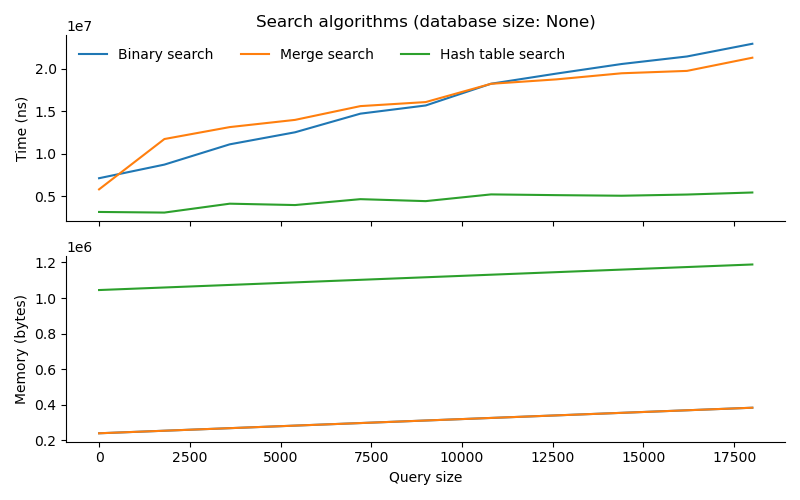
\includegraphics[width=0.6\textwidth]{./doc/db20000_qp90_r30.png}
    \caption{The empirical runtime and memory usage of search algorithm
    considering a database with 20,000 strings and a varying percentage 
    of string queries( Experiment 2).}
    \label{fig:experiment2}
\end{figure}

\begin{figure}[ht]
    \centering
    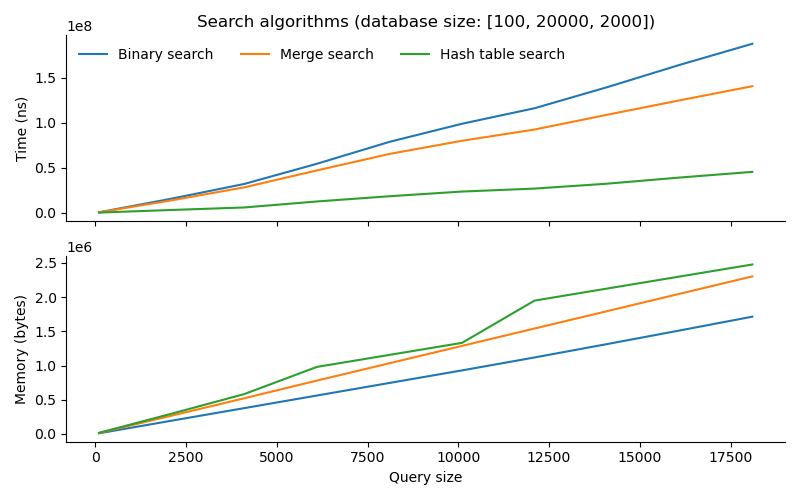
\includegraphics[width=0.5\textwidth]{./doc/db100-20000-200qp10.png}
    \caption{The empirical runtime and memory usage of search algorithm
    considering a consistent query size of 10\% of an increasingly 
    sized database (Experiment 1).}
    \label{fig:experiment1}
\end{figure}

%%%% Add your figure here %%%%

\section{Methods}

\subsection{Empirical comparison}

We measured the time and memory usage of binary, merge, and
hash table searches considering a database of 20,000 strings and query sets
ranging from 10-90\% of the query size. Strings for the database and query sets
were drawn randomly from a word list without replacement. We created a new database 
and query set for each query set size and ran each search method, recording the run 
time and memory usage separately. We repeated this step thirty times and retained 
the mean time and memory metrics.

We then measured the same attributes of the same algorithms using a set query 
percentage of 10\% of the database size which increased by 2000 from 100 to 20,000 
strings.

\subsection{Reproducibility}

To replicate these experiments, clone the repository and then run experiments 1 and 2 as follows:
\begin{verbatim}
$ clone https://github.com/audreyw04/search.git
$ cd search
$ python src/search.py \
    --experiment_number 1 \
    --query_percent 10 \
    --database_range 100 20000 2000 \
    --values_file ./data/words.txt.gz \
    --rounds 30 \
    --out_file ../doc/db100-20000-200qp10.png 
$ python ./src/search.py \
    --experiment_number 2 \
    --query_percent 90 \
    --values_file ./data/words.txt.gz \
    --rounds 30 \
    --out_file ../doc/db20000_qp90_r30.png
\end{verbatim}


\end{document}
